\documentclass[aps,prx,secnumarabic,amsmath,amssymb,10pt,superscriptaddress]{revtex4-2}
\usepackage{amsmath}
\usepackage{amssymb}
\usepackage{amsfonts}
\usepackage{color}
\usepackage{graphics}
\usepackage[pdftex]{graphicx}
\usepackage[utf8x]{inputenc}
\usepackage[colorlinks=true]{hyperref}
\usepackage{listings}
\usepackage{braket}
\usepackage{xcolor}
\newcommand\jmh[1]{{\color{magenta} #1}}

\newcommand{\ud}{\mathrm{d}}
\newcommand{\ue}{\mathrm{e}}
\newcommand{\ui}{\mathrm{i}}
\newcommand{\res}{\mathrm{Res}}
\newcommand{\Tr}{\mathrm{Tr}}
\newcommand{\dsum}{\displaystyle\sum}
\newcommand{\dprod}{\displaystyle\prod}
\newcommand{\dlim}{\dispqlaystyle\lim}
\newcommand{\dint}{\displaystyle\int}
\newcommand{\fsno}[1]{{\!\not\!{#1}}}
\newcommand{\texp}[2]{\ensuremath{{#1}\times10^{#2}}}
\newcommand{\dexp}[2]{\ensuremath{{#1}\cdot10^{#2}}}
\newcommand{\eval}[2]{{\left.{#1}\right|_{#2}}}
\newcommand{\paren}[1]{{\left({#1}\right)}}
\newcommand{\lparen}[1]{{\left({#1}\right.}}
\newcommand{\rparen}[1]{{\left.{#1}\right)}}
\newcommand{\abs}[1]{{\left|{#1}\right|}}
\newcommand{\sqr}[1]{{\left[{#1}\right]}}
\newcommand{\crly}[1]{{\left\{{#1}\right\}}}
\newcommand{\angl}[1]{{\left\langle{#1}\right\rangle}}
\newcommand{\tpdiff}[4][{}]{{\paren{\frac{\partial^{#1} {#2}}{\partial {#3}{}^{#1}}}_{#4}}}
\newcommand{\tpsdiff}[4][{}]{{\paren{\frac{\partial^{#1}}{\partial {#3}{}^{#1}}{#2}}_{#4}}}
\newcommand{\pdiff}[3][{}]{{\frac{\partial^{#1} {#2}}{\partial {#3}{}^{#1}}}}
\newcommand{\diff}[3][{}]{{\frac{\ud^{#1} {#2}}{\ud {#3}{}^{#1}}}}
\newcommand{\psdiff}[3][{}]{{\frac{\partial^{#1}}{\partial {#3}{}^{#1}} {#2}}}
\newcommand{\sdiff}[3][{}]{{\frac{\ud^{#1}}{\ud {#3}{}^{#1}} {#2}}}
\newcommand{\tpddiff}[4][{}]{{\left(\dfrac{\partial^{#1} {#2}}{\partial {#3}{}^{#1}}\right)_{#4}}}
\newcommand{\tpsddiff}[4][{}]{{\paren{\dfrac{\partial^{#1}}{\partial {#3}{}^{#1}}{#2}}_{#4}}}
\newcommand{\pddiff}[3][{}]{{\dfrac{\partial^{#1} {#2}}{\partial {#3}{}^{#1}}}}
\newcommand{\ddiff}[3][{}]{{\dfrac{\ud^{#1} {#2}}{\ud {#3}{}^{#1}}}}
\newcommand{\psddiff}[3][{}]{{\frac{\partial^{#1}}{\partial{}^{#1} {#3}} {#2}}}
\newcommand{\sddiff}[3][{}]{{\frac{\ud^{#1}}{\ud {#3}{}^{#1}} {#2}}}
\newcommand{\eff}{ef\! f}

\newcommand{\todo}[1]{}

\newcommand{\harvardphysics}{\affiliation{Department of Physics, Harvard University, Cambridge, Massachusetts 02138, USA}}
\newcommand{\harvardccb}{\affiliation{Department of Chemistry and Chemical Biology, Harvard University, Cambridge, Massachusetts 02138, USA}}
\newcommand{\cua}{\affiliation{Harvard-MIT Center for Ultracold Atoms, Cambridge, Massachusetts 02138, USA}}
\newcommand{\gradstudent}{
  \harvardphysics
  \harvardccb
  \cua
}
\newcommand{\itamp}{\affiliation{ITAMP, Harvard-Smithsonian Center for Astrophysics, Cambridge, Massachusetts 02138, USA}}

% Add S1 to bibliography
\renewcommand*{\citenumfont}[1]{S#1}
\renewcommand*{\bibnumfmt}[1]{[S#1]}

% Add S to labels
\setcounter{table}{0}
\renewcommand{\thetable}{S\arabic{table}}%
\setcounter{figure}{0}
\renewcommand{\thefigure}{S\arabic{figure}}%
\renewcommand{\thepage}{S\arabic{page}}
\renewcommand{\thesection}{S\arabic{section}}
\renewcommand{\theequation}{S.\arabic{equation}}

\ifpdf
% Ensure reproducible output
\pdfinfoomitdate=1
\pdfsuppressptexinfo=-1
\pdftrailerid{}
\hypersetup{
  pdfcreator={},
  pdfproducer={}
}
\fi

\begin{document}
\title{Coherent optical creation of a single molecule -- Supplemental material}
\author{Yichao~Yu}
\thanks{Y.Y.~and K.W.~contributed equally to this work.}
\email{yichaoyu@g.harvard.edu}
\gradstudent
\author{Kenneth~Wang}
\thanks{Y.Y.~and K.W.~contributed equally to this work.}
\gradstudent
\author{Jonathan~D.~Hood}
\affiliation{Department of Chemistry, Purdue University, West Lafayette, Indiana, 47906, USA}
\author{Lewis~R.~B.~Picard}
\gradstudent
\author{Jessie~T.~Zhang}
\gradstudent
\author{William~B.~Cairncross}
\harvardccb
\harvardphysics
\cua
\author{Jeremy~M.~Hutson}
\affiliation{Joint Quantum Centre Durham-Newcastle, Department of Chemistry, Durham University, Durham, DH1 3LE, United Kingdom}
\author{Rosario Gonzalez-Ferez}
\affiliation{Instituto Carlos I de F\'{\i}sica Te\'orica y Computacional, and Departamento de F\'{\i}sica At\'omica, Molecular y Nuclear,  Universidad de Granada, 18071 Granada, Spain}
\itamp
\author{Till Rosenband}
\affiliation{Agendile LLC, Cambridge, Massachusetts 02139, USA}
\author{Kang-Kuen~Ni}
\email{ni@chemistry.harvard.edu}
\harvardccb
\harvardphysics
\cua

\date{\today}

\maketitle

\section{3 Level Raman Transfer with Cross Coupling}

In our system, the separation in energy between the initial and target state is much smaller than the single photon detuning $\Delta$ from the intermediate state; see Fig.~1a in the main text.
Thus, there is significant cross coupling for the scattering rate and light shift, where each state is coupled to the excited state by the power in both beams.
Under these conditions, the scattering rate and light shift are proportional to the total power $P_{\text{tot}} = P_{\rm m} + P_{\rm a}$, where $P_{\rm m} (P_{\rm a})$ is the power in the beam that addresses the molecular (atomic) state.
The Raman Rabi frequency is proportional to $\sqrt{P_{\rm m}P_{\rm a}} $.
With a fixed total power and thus fixed scattering rate, the Raman Rabi frequency is maximized when $ P_{\rm m} = P_{\rm a} = P_{\text{tot}}/2$.

For the purposes of this work, we denote $\Omega_{\rm a} $($\Omega_{\rm m}$) as the Rabi frequencies to drive a transition from the atom (target molecule) state to the intermediate state used in the Raman transition corresponding to the power in a single beam, $P_{\rm a}$ ($P_{\rm m}$).
Thus, the Raman Rabi frequency is $\Omega_{\rm a}\Omega_{\rm m}/(2\Delta)$, where $ \Delta $ is the single photon detuning.
Cross coupling affects the scattering rate and light shift, and assuming equal powers in both beams, these quantities become $ \Gamma_{\rm e} \Omega_{\rm m}^2 / (2\Delta^2) + \Gamma_{\rm e} \Omega_{\rm a}^2 / (2\Delta^2) $ and $ \Omega_{\rm m}^2/(2\Delta) - \Omega_{\rm a}^2/(2\Delta) $, where $\Gamma_{\rm e}$ is the excited state linewidth. Since $ \Omega_{\rm m} >> \Omega_{\rm a} $, the scattering rate and light shift can be approximated as $ \Gamma_{\rm e} \Omega_{\rm m}^2/(2\Delta^2)$ and $\Omega_{\rm m}^2/(2\Delta)$.

\section{Raman Transfer with Many Intermediate States} \label{sm:sect_2}
With multiple intermediate states, the total Raman Rabi frequency, scattering rate, and light shift become a sum over all these possible states. In our model, we consider all vibrational states of $ \mathrm{c^3\Sigma^+(\Omega = 1)} $ and states in the atomic continuum as intermediate states. The Rabi frequency between two states is proportional to the electronic dipole moment, arising from the electronic wavefunctions, and the overlap of the vibrational wavefunctions. Under the assumption that the electronic dipole moment $ d $ is the same for all transitions between the ground state and the excited electronic state, the total Raman Rabi frequency becomes
\begin{equation}
  \Omega_{\rm R} = \frac{d^2E^2}{2\hbar^2} \displaystyle\sum_{v'} \frac{\braket{a|v'}\braket{v'|m}}{\Delta_{v'}},
\end{equation}
where $\ket{a}$ ($\ket{m}$) are the relative coordinate wavefunctions for the trapped atomic (target molecular) state, and $\ket{v'}$ is the relative-coordinate wavefunction for the excited state which includes both bound molecular states and the atomic continuum. $\Delta_{v'}$ is a single photon detuning with respect to the $\ket{v'}$ state, $ E $ is the electric field for the power in the single beam given a waist size. We can divide this sum into a sum over all the bound molecular states, and a sum over atomic continuum states,
\begin{equation}
  \Omega_{\rm R} = \frac{d^2E^2}{2\hbar^2}\displaystyle\sum_{v' \leq v'_{\text{max}}} \frac{\braket{a|v'}\braket{v'|m}}{\Delta_{v'}} +  \frac{d^2E^2}{2\hbar^2}\displaystyle\sum_{v' > v'_{\text{max}}} \frac{\braket{a|v'}\braket{v'|m}}{\Delta_{v'}},
\end{equation}
where $ v'_{\text{max}}$ corresponds to the excited molecular state, which is most weakly bound. The first term can be calculated numerically given an excited state potential. To calculate the second term, we first make an assumption that we are far enough detuned from the contributing continuum states that they are all at approximately the same detuning, $ \Delta_{\text{thresh}}$. This allows us to pull it out of the sum, and we obtain
\begin{equation}
  \Omega_{\rm R} \approx \frac{d^2E^2}{2\hbar^2}\displaystyle\sum_{v' \leq v'_{\text{max}}} \frac{\braket{a|v'}\braket{v'|m}}{\Delta_{v'}} +  \frac{d^2E^2}{2\hbar^2\Delta_{\text{thresh}}}\displaystyle\sum_{v' > v'_{\text{max}}} \braket{a|v'}\braket{v'|m} . \label{rabifreq}
\end{equation}
From requiring completeness and orthogonality,
\begin{equation}
  \displaystyle\sum_{v'} \braket{a|v'}\braket{v'|m} = \braket{a|m} = 0,
\end{equation}
we derive an expression for the second sum in equation \ref{rabifreq}
\begin{equation}
  \displaystyle\sum_{v'> v'_{\text{max}}} \braket{a|v'}\braket{v'|m} = -\displaystyle\sum_{v' \leq v'_{\text{max}}} \braket{a|v'}\braket{v'|m},
\end{equation}
which can be calculated from the vibrational states of the excited state potential. Thus, the Raman Rabi frequency can be approximated as:
\begin{equation}
  \Omega_{\rm R} \approx \frac{d^2E^2}{2\hbar^2}\displaystyle\sum_{v' \leq v'_{\text{max}}} \frac{\braket{a|v'}\braket{v'|m}}{\Delta_{v'}} -  \frac{d^2E^2}{2\hbar^2\Delta_{\text{thresh}}}\displaystyle\sum_{v' \leq v'_{\text{max}}} \braket{a|v'}\braket{v'|m}.
\end{equation}
We can account for the atomic continuum in the scattering rate in a similar way
\begin{align}
  \Gamma_{\rm s} &\approx \frac{d^2E^2}{2\hbar^2}\displaystyle\sum_{v' \leq v'_{\text{max}}}\Gamma_{v'} \frac{\braket{m|v'}\braket{v'|m}}{\Delta_{v'}^2} + \frac{d^2E^2\Gamma}{2\hbar^2\Delta_{\text{thresh}}^2}\displaystyle\sum_{v' > v'_{\text{max}}}\braket{m|v'}\braket{v'|m},
\end{align}
where $\Gamma_{v'}$ is the excited state linewidth for the $\ket{v'}$ state, and we have assumed the atomic continuum states all have the same linewidth $\Gamma$. Using normalization, we derive an expression for the sum in the second term
\begin{equation}
  \displaystyle\sum_{v' > v'_{\text{max}}}\braket{m|v'}\braket{v'|m} = 1 - \displaystyle\sum_{v' \leq v'_{\text{max}}}\braket{m|v'}\braket{v'|m}.
\end{equation}
We then arrive at an expression for the scattering rate, accounting for the atomic continuum,
\begin{equation}
  \Gamma_{\rm s} \approx \frac{d^2E^2}{2\hbar^2}\displaystyle\sum_{v' \leq v'_{\text{max}}}\Gamma_{v'} \frac{\braket{m|v'}\braket{v'|m}}{\Delta_{v'}^2} +  \frac{d^2E^2\Gamma}{2\hbar^2\Delta_{\text{thresh}}^2}\left(1 - \displaystyle\sum_{v' \leq v'_{\text{max}}}\braket{m|v'}\braket{v'|m}\right).
\end{equation}
We have replaced the full continuum with an effective state at the atomic threshold with strength proportional to the amount of wavefunction overlap between the target molecular state and all atomic continuum states. This model leads to a component in the scattering rate that is proportional to $ 1/\Delta_{\text{thresh}}^2$ and is smaller as one detunes farther from the threshold. We note that the first term can also scale nearly as $1/\Delta_{\text{thresh}}^2 $, if, as in our case, the largest terms in the summation are from states near the threshold.

A very similar result holds for the light shift $\delta$ and is written here for completeness

\begin{equation}
  \delta = \frac{d^2E^2}{2\hbar^2}\displaystyle\sum_{v' \leq v'_{\text{max}}} \frac{\braket{m|v'}\braket{v'|m}}{\Delta_{v'}} +  \frac{d^2E^2}{2\hbar^2\Delta_{\text{thresh}}}\left(1 - \displaystyle\sum_{v' \leq v'_{\text{max}}}\braket{m|v'}\braket{v'|m}\right).
\end{equation}

\section{Computational methods for bound and scattering states}

For scattering and near-threshold bound states, we solve the Schr\"odinger equation by
coupled-channel methods \cite{HUTSON1994}, using a basis set in which the electron spins
$s_{\rm Na}$ and $s_{\rm Cs}$ and the nuclear spins $i_{\rm Na}$ and $i_{\rm Cs}$ are separately
coupled,
\begin{equation}
  | (s_{\rm Na} s_{\rm Cs} S)
  (i_{\rm Na} i_{\rm Cs} I) F M_F\rangle.
  \label{eqbassif}
\end{equation}
Here $S$ and $I$ are the total electron and nuclear spins of the molecule or atomic pair. Their
resultant $F$ is the total spin, with projection $M_F$ onto the axis of the magnetic field. In
principle $F$ can be further coupled to the rotational angular momentum $L$, but in the present
work only functions with $L=0$ are included. In the absence of a magnetic field, $F$ and $M_F$ are
both good quantum numbers, but in a magnetic field only $M_F$ is conserved. The calculations in
this paper use basis sets with all possible values of $S$, $I$ and $F$ (for the required value of
$M_F$) that can be constructed with $s_{\rm Na} = s_{\rm Cs} = 1/2$,
$i_{\rm Na} = 3/2$ and $i_{\rm Cs} = 7/2$.

Scattering calculations are carried out using the MOLSCAT package \cite{molscat:2019,
  mbf-github:2020} and bound-state calculations using the related BOUND package
\cite{bound+field:2019, mbf-github:2020}. The calculations use singlet and triplet interaction
potentials for Na+Cs obtained by adjusting the potentials of Docenko \emph{et al.}\
\cite{Docenko2006} at short range, using the same procedure as for KCs \cite{Groebner2017},
to reproduce the experimental binding energy of the least-bound triplet state \cite{Hood2019}
and the position of the s-wave Feshbach resonance near 864~G \cite{Zhang2020}. The atomic
nuclear hyperfine coupling and Zeeman effects are fully included, using the Hamiltonian described
in \cite{Hutson2008}.

The bound-state calculations were initially used to predict the binding energies of states that lie
within about 1~GHz of each atomic threshold of interest. At zero magnetic field, the states fall
into groups from each hyperfine state of the atomic pair, labeled by $(f_{\rm Na},f_{\rm Cs})$. For
example, for the $(f_{\rm Na},f_{\rm Cs}) = (2,3)$ states that are of principal interest here, each
group comprises 5 zero-field levels with $F=1,2,3,4$ and 5; one such group is spread out over a
range of energies between 290 MHz and 770 MHz below the $(f_{\rm Na},f_{\rm Cs}) = (2,3)$
threshold. In a magnetic field, each zero-field level splits into $2F+1$ Zeeman sublevels labeled
by $M_F$. For each sublevel we can calculate the dependence of the energy on magnetic field, in
order to choose a target state for which the Raman transition frequency depends only weakly on
field.

The state that we ultimately chose as the target state for Raman transfer is the least-bound
$(F,M_F)=(5,5)$ sublevel with $(f_{\rm Na},f_{\rm Cs}) = (2,3)$, which was predicted at a binding
energy 763 MHz below the $(f_{\rm Na},f_{\rm Cs}) = (2,3)$ threshold. As described in the text, it
was subsequently located experimentally at a binding energy of 770.57150(9) MHz.

Multichannel bound-state wavefunctions, with components labeled by $S$, $I$ and $F$, are calculated
using the method of Thornley and Hutson \cite{Thornley1994}. For molecular bound states, they are
obtained on a grid of internuclear distances from 2.4~\AA\ to 50~\AA. For states of confined atomic
pairs, a harmonic confining potential is added to the molecular potentials and the grid is extended
to 3000~\AA.

\section{Excited Molecular States} \label{sm:excited_states}
To obtain a full calculation for the expected Raman Rabi frequency, light shift and scattering, we need to account for all the excited molecular states.
The lowest eight excited molecular potentials in NaCs asymptote to the dissociation limit of Na 3S + Cs 6P.
These eight potentials can be written in the Hund's case (a) basis as $ \mathrm{c^3\Sigma^+_{\Omega = 0^-},c^3\Sigma^+_{\Omega = 1}, b^3\Pi_{\Omega = 0^-}, b^3\Pi_{\Omega = 0^+}, b^3\Pi_{\Omega = 1}, b^3\Pi_{\Omega = 2}, B^1\Pi_{\Omega = 1}, A^1\Sigma^+_{\Omega = 0^+}}$ \cite{Korek2007}.
Due to spin-orbit coupling, especially large in Cs, the excited molecular states are mixed, containing components in multiple potentials.
Fortunately, single-channel potential energy curves for $\mathrm{c^3\Sigma^+_1}$ and $  B^1\Pi_1 $ have been experimentally determined, and are predictive across the entire energy range of the potential \cite{Grochola2010, Grochola2011, Liu2017}.
Since there is only one $ \Omega = 2$ potential at this dissociation limit, a single-channel potential has been determined for $ b^3\Pi_2$ as well \cite{Zabawa2012}.
Unfortunately, single-channel potentials for the other electronic states do not exist.
A deperturbation analysis was required for states belonging to the mixed $\mathrm{A-b}$ complex,
and the fitted potentials and spin-orbit coupling coefficients are only accurate within the energy range of the measured experimental data \cite{Zaharova2009}.
Since our experiment attempts to work in a regime where the predominant Raman coupling comes from the $v' = 0$ state of $ \mathrm{c^3\Sigma^+_1} $,
the contribution of the other seven potentials is mainly to a background that is nearly detuning independent.
Thus, for computational ease, we use the diabatic potentials for $ \mathrm{b^3\Pi_{0}, b^3\Pi_{1}} $ and $ \mathrm{A^1\Sigma^+_{0^+}}$.
% and remove the states nearest to the $ v' = 0$ state of $ \mathrm{c^3\Sigma^+_1} $.
Lastly, to our knowledge, no potential fit to experimental data exists for the $ c^3\Sigma^+_{0^-}$ state. Assuming that its contribution is only to the background, as an approximation, we simply double the contribution of all states except $v' = 0$ from $ c^3\Sigma^+_1$.

\section{Calculating Matrix Elements with Coupled Channel Ground State}
To calculate Rabi frequencies for transitions to the eight excited molecular potentials, we
obtain their wavefunctions from a single-channel calculation \cite{Fattal1996} using the potential energy curves described in section \ref{sm:excited_states}. We
then calculate overlap integrals between these functions and either the triplet ($S=1$) or singlet ($S=0$) components of the
coupled-channel wavefunctions for either the target molecular state or the confined atomic state.
These calculations assume that the intermediate states have pure singlet or triplet character and neglect its
nuclear spin character, which is unknown. These calculations include theoretical electronic transition dipole moments~\footnote{Private communication with R. Moszynski}.

The full calculation of the Raman Rabi frequency and scattering rate using the methods in section \ref{sm:sect_2} is shown in figure \ref{f-sm}. The strong contribution from the atomic threshold arises from the large overlap to the near-threshold bound states shown in figure \ref{f-smfcf} for the $c^3\Sigma^+_1$ state. This leads to a $1/\Delta_{\text{thresh}}^2$ dependence of the scattering rate and favors using deeply bound states as the intermediate state for the Raman transfer. A similar result holds for the other excited state potentials.



\begin{figure}[ht!]
  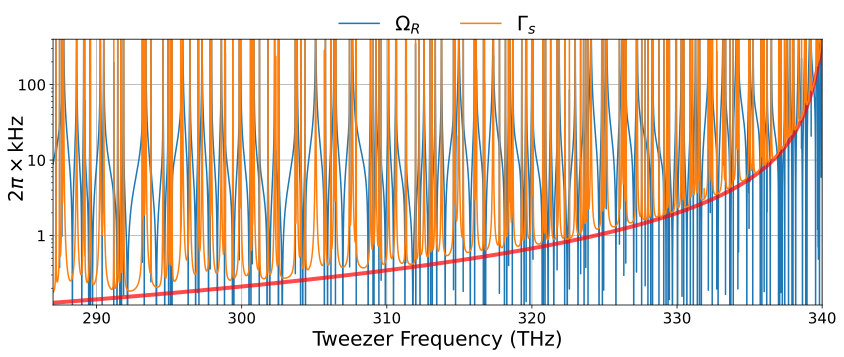
\includegraphics[width=\textwidth]{imgs/raman_theory_full.pdf}
  \caption{Full calculation of the Raman Rabi frequency and scattering rate
    as a function of the single-photon frequency
    including all vibrational states of $ \mathrm{c^3\Sigma^+(\Omega = 1)}$
    and the atomic continuum.
    The second frequency in the Raman transition is offset by about $770~\mathrm{MHz}$
    and resonant with the two photon transition.
    The assumed excited-state linewidth for all molecular lines is $50~\text{MHz}$.
    The red line shows the contribution that comes only from the near-threshold states.
    \label{f-sm}}
\end{figure}

\begin{figure}[ht!]
  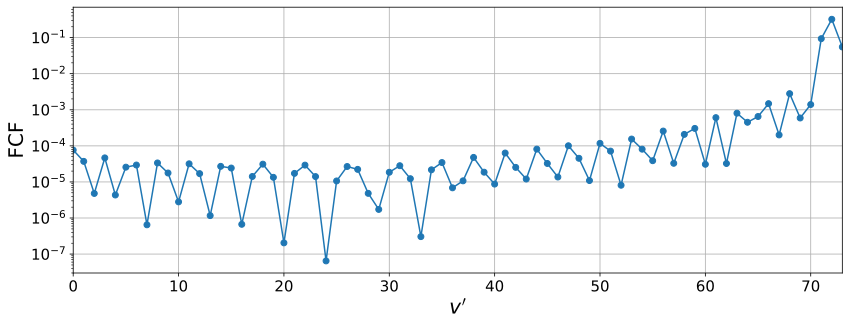
\includegraphics[width=\textwidth]{imgs/fcf_c3sigma.pdf}
  \caption{The Franck-Condon Factor (FCF) between the target molecular state and vibrational state $v'$ of $c^3\Sigma^+_1$. The potential supports 74 bound states, and the predominant contribution arises from the near-threshold bound states. The total overlap with all the bound states is $0.4822$, which is $96.8\%$ of the total triplet fraction of the target molecular state.
    \label{f-smfcf}}
\end{figure}
\section{Effective Matrix Elements to a Single State}

In this calculation, there is a matrix element, $\Omega_{\mathrm{a}ij}, \Omega_{\mathrm{m}ij}$ between each channel $ i $ of the coupled channel ground state and an excited state $ j $. The total Raman Rabi frequency $ \Omega_{\rm R}$, light shift $ \delta$ and off-resonant scattering $ \Gamma_{\rm s} $ contribution from this single excited state is calculated as

\begin{align}
  \Omega_{\mathrm{R}j} &= \displaystyle\sum_{i} \frac{\Omega_{\mathrm{a}ij} \Omega_{\mathrm{m}ij}}{2\Delta}, \\
  \delta_j &= \displaystyle\sum_{i} \frac{\Omega_{\mathrm{a}ij}^2 - \Omega_{\mathrm{m}ij}^2}{2\Delta}, \\
  \Gamma_{\mathrm{s} j} &= \displaystyle\sum_{i} \Gamma_{\rm e} \frac{\Omega_{\mathrm{a}ij}^2 + \Omega_{\mathrm{m}ij}^2}{2\Delta^2},
\end{align}
where $ \Delta $ is the single photon detuning and $ \Gamma_{\rm e} $ is the excited state linewidth. The experiment, through measuring the detuning dependence of the Raman Rabi frequency and the resonance frequency, extracts a single $ \Omega_{\rm m} $ and $ \Omega_{\rm a} $. In order to compare to the theory, we introduce effective $ \Omega_{\rm a}', \Omega_{\rm m}', \Gamma_{\rm e}'$, so that $ \Omega_{\rm R} = \Omega_{\rm a}'\Omega_{\rm m}'/(2\Delta) $, $\delta = (\Omega_{\rm a}'^2 - \Omega_{\rm m}'^2)/(2\Delta) $, and $\Gamma_{\rm s} = \Gamma_{\rm e}'(\Omega_{\rm a}'^2 + \Omega_{\rm m}'^2)/(2\Delta^2) $. The effective Rabi frequencies for the $v' = 0$ state of $ c^3\Sigma^+_1$ and their ratio are reported in Table~\ref{tab:sm} at $3.75~\mathrm{mW}$ of tweezer power.

% $2\pi \times 15.3~\mathrm{kHz}$
% $ 2\pi \times 533~\mathrm{Hz}$
% $2\pi \times 573 ~\mathrm{MHz}$
% $2\pi \times 7.37 ~\mathrm{MHz}$

\begin{table}[ht]
  \centering
  \begin{tabular}{|c|c|} \hline
    $\Omega_{\rm m}'$ &  $2\pi \times 573 ~\mathrm{MHz}$ \\
    $\Omega_{\rm a}'$ &  $2\pi \times 7.37 ~\mathrm{MHz}$ \\
    $\Omega_{\rm a}'/\Omega_{\rm m}'$ & $ 0.013 $ \\ \hline
  \end{tabular}
  \caption{ The effective Rabi frequencies for the $v' = 0$ state of $c^3\Sigma^+_1$ at $ 3.75~\mathrm{mW}$ of tweezer power.
    \label{tab:sm}}
\end{table}


\section{Scaling of atomic matrix element with tweezer power}

Since our coupled-channel calculations include the harmonic confinement, we can calculate the enhancement in $\Omega_{\rm a}$ with increasing confinement. Using two calculations with $ \omega_{\text{trap}} = 36.5~\mathrm{kHz}$ and $\omega_{\text{trap}} = 80~\mathrm{kHz}$ trapping frequencies, and assuming a power law scaling, we find that the wavefunction overlap scales as $ \omega_{\text{trap}}^{0.58} = P^{0.29} $. Thus, $\Omega_{\rm a} \propto P^{0.79} $, which was also experimentally verified. However, we note that in the actual experiment, our system does not have spherically symmetric confinement. The radial trapping frequency is about $5.7$ times larger than the axial trapping frequency.
\todo{
  Power/intensity calibration
}

\bibliography{master_ref}
\end{document}
